
%%% distributed:
% shared memory not enough, mkl, nautilus/kraken

%%% What is a supercomputer? (interconnect)

% \section{Supercomputers}

% \hidenum
% \begin{frame}[noframenumbering]
% \frametitle{Contents}
%  \tableofcontents[currentsection,hideallsubsections]
% \end{frame}
% \shownum



% \subsection{Supercomputing}

\begin{frame}
  \begin{block}{Shared and Distributed Memory Machines}
   \begin{center}
    \begin{minipage}{.475\textwidth}
    \begin{block}{Shared Memory}
     Direct access to read/change memory (one node)
      \begin{center}
      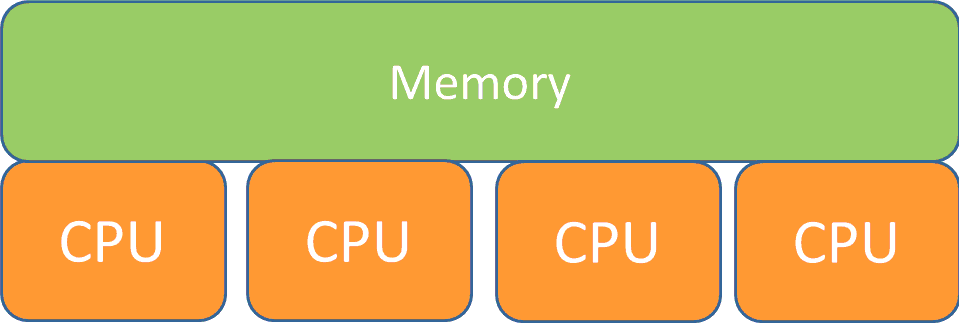
\includegraphics[width=.95\textwidth]{pics/arch_shared}
      \end{center}
      \vspace{.3cm} \
    \end{block}
    \end{minipage}
    \hspace{.1cm}
    \begin{minipage}{.475\textwidth}
    \begin{block}{Distributed}
    No direct access to read/change memory.
      \begin{center}
      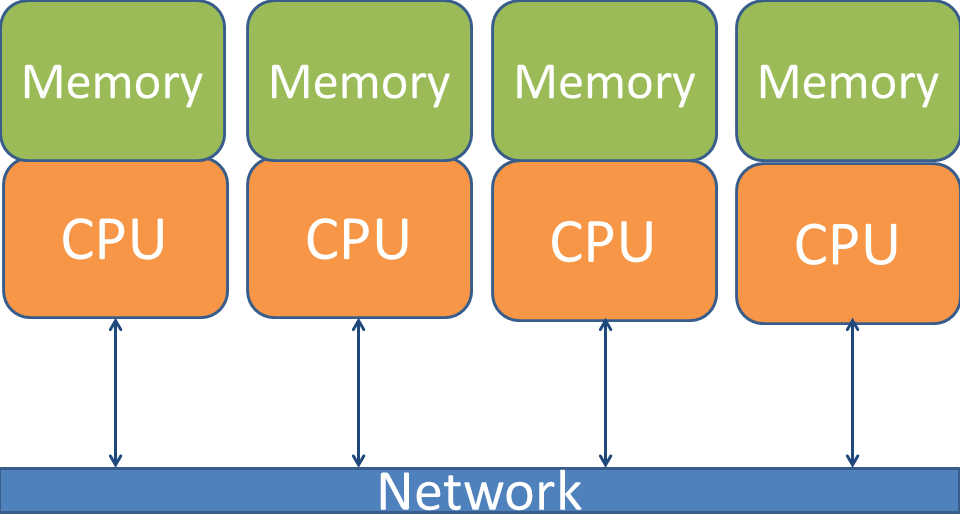
\includegraphics[width=.95\textwidth]{pics/arch_distributed}
      \end{center}
    \end{block}
    \end{minipage}
    \end{center}
    \end{block}
\end{frame}


\begin{frame}
  \begin{block}{Shared and Distributed Memory Machines}
   \begin{center}
    \begin{minipage}[t]{.47\textwidth}
    \begin{block}{Shared Memory Machines}
    \begin{center}
    Thousands of cores\\[.2cm]
    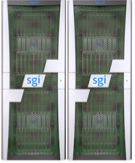
\includegraphics[scale=.65]{pics/nautilus}\\
    {\tiny \emph{Nautilus}, University of Tennessee\\1024 cores \\4 TB RAM\\}
    \end{center}
    \end{block}
    \end{minipage}
    \hspace{.1cm}
    \begin{minipage}[t]{.47\textwidth}
    \begin{block}{Distributed Memory Machines}
    \begin{center}
    Hundreds of thousands of cores\\[.2cm]
    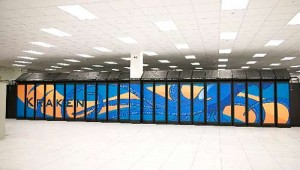
\includegraphics[width=.95\textwidth]{pics/kraken}\\
    {\tiny \emph{Kraken}, University of Tennessee\\ 112,896 cores \\147 TB RAM\\}
    \end{center}
    \end{block}
    \end{minipage}
    \end{center}
    \end{block}
\end{frame}



% \begin{frame}
% \frametitle{MKL Benchmark on $\approx 0.75$ GiB}
% \begin{center}
%     \hspace*{-1cm}\includegraphics[width=1.2\textwidth]{pics/rbenchmarkplotMatrix}  
% \end{center}
% \end{frame}


% \begin{frame}
%   \begin{block}{Terminology: Difficulty in Parallelism}
%     \begin{enumerate}[<+-|alert@+>]
%       \item \emph{Embarrassingly parallel}: easy/trivial to make parallel.
%       \item \emph{Tightly coupled}: difficult to make parallel.
%     \end{enumerate}
%   \end{block}
% \end{frame}



